\hypertarget{barcode_8inc}{
\section{include/barcode.inc File Reference}
\label{barcode_8inc}\index{include/barcode.inc@{include/barcode.inc}}
}
Functions for the handling of different barcodes. 

\subsection*{Functions}
\begin{CompactItemize}
\item 
\hyperlink{barcode_8inc_6d3645af0ef526e4f64d28dcbdceb74f}{checkBarcode} (\$barcode)
\item 
\hyperlink{barcode_8inc_e10c37e4f9f9b7c6617a388351a27c99}{getBarcodeInfo} (\$barcode)
\end{CompactItemize}


\subsection{Detailed Description}
Functions for the handling of different barcodes. 

This file currently deals with the handling of barcodes and getting the information associated with them. 

Definition in file \hyperlink{barcode_8inc-source}{barcode.inc}.

\subsection{Function Documentation}
\hypertarget{barcode_8inc_6d3645af0ef526e4f64d28dcbdceb74f}{
\index{barcode.inc@{barcode.inc}!checkBarcode@{checkBarcode}}
\index{checkBarcode@{checkBarcode}!barcode.inc@{barcode.inc}}
\subsubsection{\setlength{\rightskip}{0pt plus 5cm}checkBarcode (\$ {\em barcode})}}
\label{barcode_8inc_6d3645af0ef526e4f64d28dcbdceb74f}


Checks to see if a valid, handalable, barcode was entered. \begin{Desc}
\item[Parameters:]
\begin{description}
\item[{\em \$barcode}]The Barcode to be checked \end{description}
\end{Desc}
\begin{Desc}
\item[Returns:]The type of barcode entered if valid, FALSE if it is not \end{Desc}


Definition at line 16 of file barcode.inc.

References XMLRPC\_\-prepare(), and XMLRPC\_\-request().

\begin{Code}\begin{verbatim}16                                 {
17   switch ($_GET['type']) {
18     case 'upc':
22       $result = XMLRPC_request('dev.upcdatabase.com', '/rpc', 'lookupUPC', array(XMLRPC_prepare($barcode)));
23       if ($result[1] != 'Error: Invalid length') {
24         if (strlen($barcode) == 12) {
25           return 'upca';
26         }
27         else if (strlen($barcode) == 13) {
28           return 'ean13';
29         }
30         else {
31           return FALSE;
32         }
33       }
34       else {
35         return FALSE;
36       }
37       break;
38   }
39 }
\end{verbatim}
\end{Code}




Here is the call graph for this function:\nopagebreak
\begin{figure}[H]
\begin{center}
\leavevmode
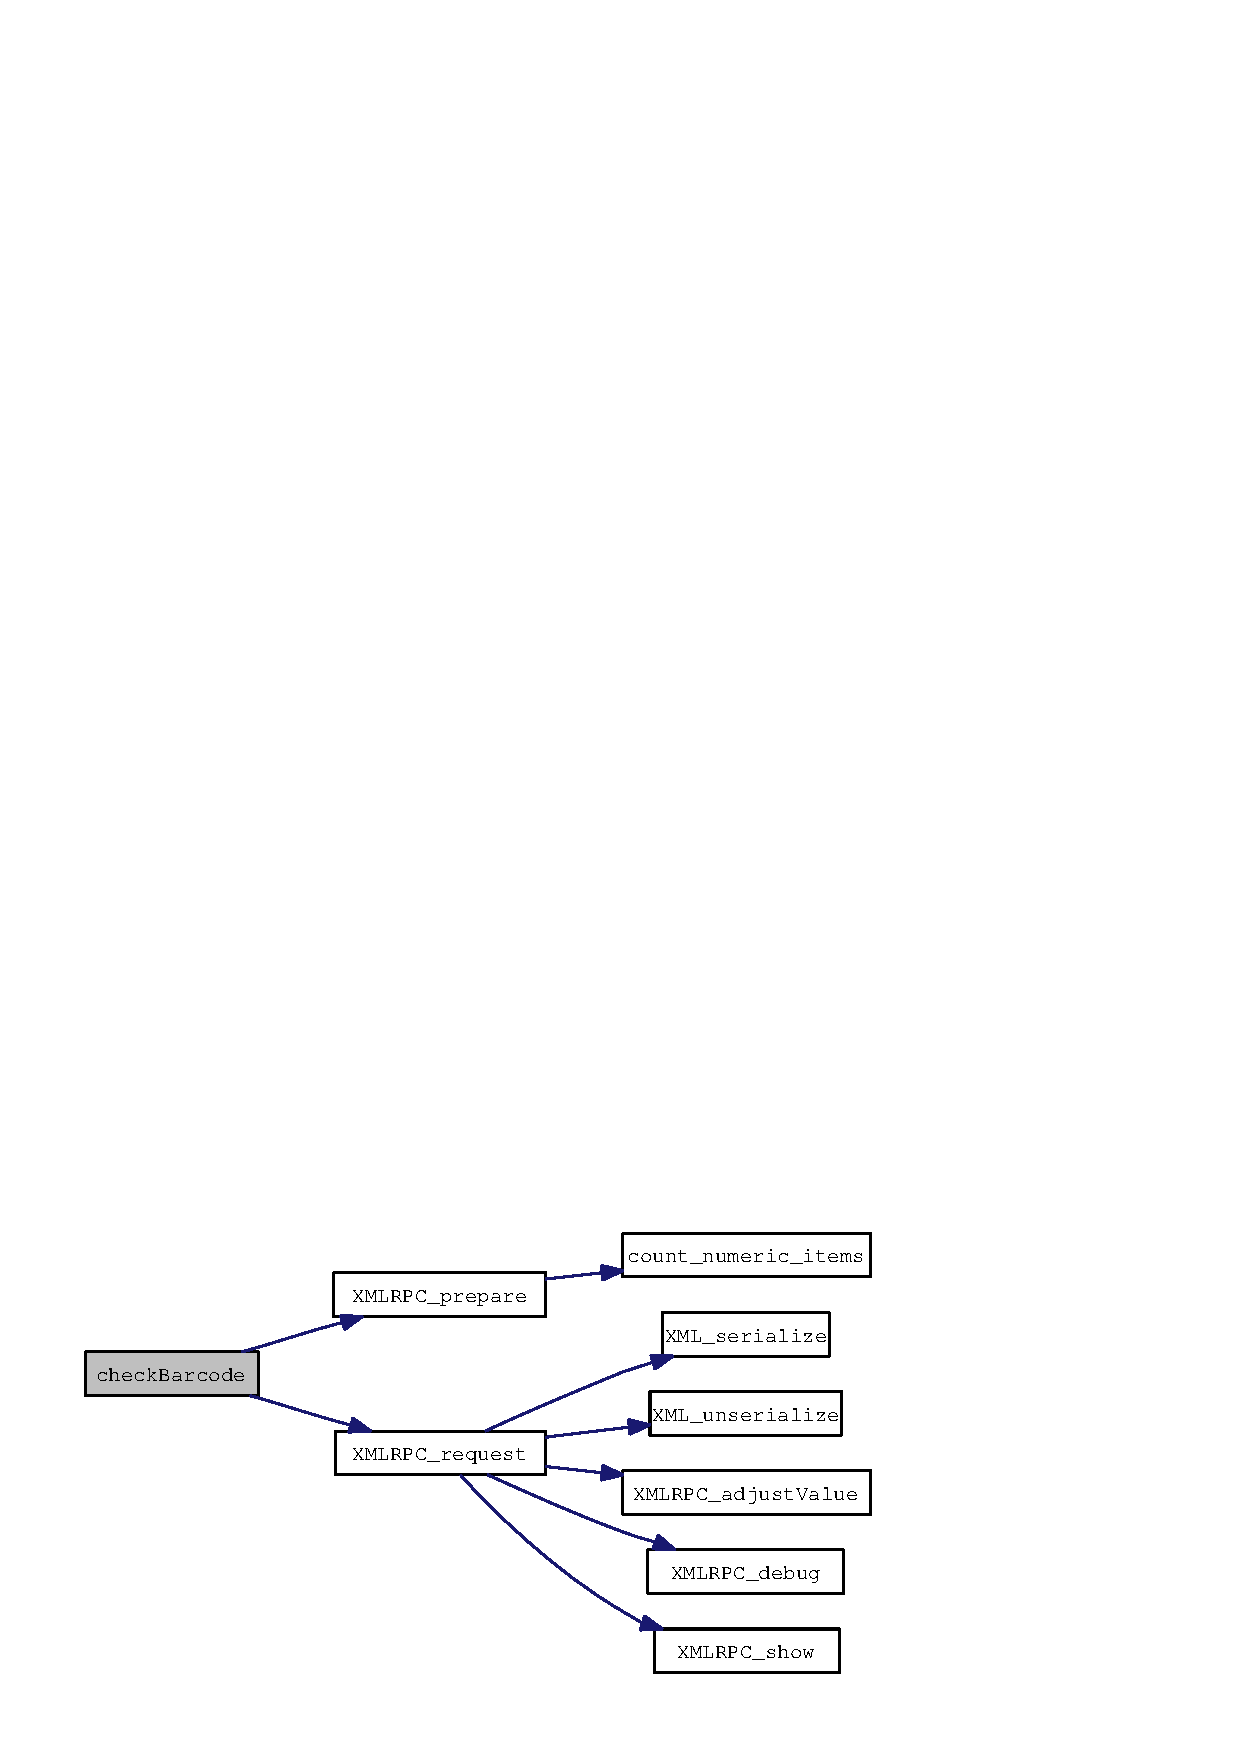
\includegraphics[width=211pt]{barcode_8inc_6d3645af0ef526e4f64d28dcbdceb74f_cgraph}
\end{center}
\end{figure}
\hypertarget{barcode_8inc_e10c37e4f9f9b7c6617a388351a27c99}{
\index{barcode.inc@{barcode.inc}!getBarcodeInfo@{getBarcodeInfo}}
\index{getBarcodeInfo@{getBarcodeInfo}!barcode.inc@{barcode.inc}}
\subsubsection{\setlength{\rightskip}{0pt plus 5cm}getBarcodeInfo (\$ {\em barcode})}}
\label{barcode_8inc_e10c37e4f9f9b7c6617a388351a27c99}


Output Barcode Info \begin{Desc}
\item[Parameters:]
\begin{description}
\item[{\em \$barcode}]The barcode to lookup \end{description}
\end{Desc}
\begin{Desc}
\item[Returns:]HTML code to create the info area \end{Desc}
\begin{Desc}
\item[See also:]\hyperlink{barcode_8inc_6d3645af0ef526e4f64d28dcbdceb74f}{checkBarcode} \end{Desc}


Definition at line 47 of file barcode.inc.

References getImages(), XMLRPC\_\-prepare(), and XMLRPC\_\-request().

\begin{Code}\begin{verbatim}47                                   {
48   switch ($_GET['type']) {
49     case 'upc':
53       $output = '';
54       $output .= '<div id="upc">';
55       $output .= '<img src="upcimg.php?upc=' . $barcode . '" />';
56       $output .= '</div>';
57 
61       $result = XMLRPC_request('dev.upcdatabase.com', '/rpc', 'lookupUPC', array(XMLRPC_prepare($barcode)));
62 //    if ($debug) var_dump($result);
63       echo getImages($result[1]['description']);
64       if ($result[1]['found']) {
65         extract($result[1], EXTR_PREFIX_ALL, 'barcode');
66         $output .= <<<_HTML
67         <div id="info">
68           <table align="center">
69             <tr>
70               <td class="title">Country</td>
71               <td>$barcode_issuerCountry</td>
72             </tr>
73             <tr>
74               <td class="title">Description</td>
75               <td>$barcode_description</td>
76             </tr>
77             <tr>
78               <td class="title">Size</td>
79               <td>$barcode_size</td>
80             </tr>
81           </table>
82           <a href="http://www.upcdatabase.com/editform.asp?upc=$barcode">Modify this entry</a>
83           <a href="http://www.upcdatabase.com/deleteform.asp?upc=$barcode">Delete this entry</a>
84         </div>
85 _HTML;
86       }
87       else {
88         $output .= 'Product Not Found!<br />';
89         $output .= '<a href="http://www.upcdatabase.com/addform.asp?upc=' . $barcode . '">Add this item to the database</a>';
90       }
91 
92       return $output;
93       break;
94   }
95 }\end{verbatim}
\end{Code}




Here is the call graph for this function:\nopagebreak
\begin{figure}[H]
\begin{center}
\leavevmode
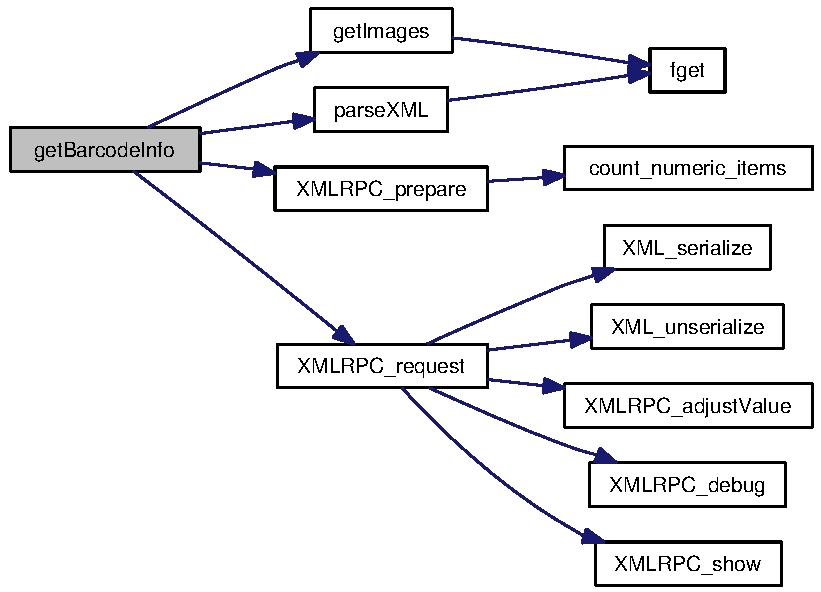
\includegraphics[width=215pt]{barcode_8inc_e10c37e4f9f9b7c6617a388351a27c99_cgraph}
\end{center}
\end{figure}
